\section{Payment gateway}
\label{sec:payment_gateway}
The world over, traditional paper based payment modes have evolved significantly to include new and efficient ADCs such as Automated Teller Machines (ATMs), Point of Sale (POS) machines, internet banking, mobile banking etc. These have transformed the very concept of banking to include sophisticated e-payment instruments, thereby making it more convenient for people to conduct transactions across the globe any time even while sitting at home \cite{payment_gateway_a}.
\newline
An important infrastructural component to facilitate the electronic transactions is establishment of a payment gateway. A payment gateway is an e-commerce application service provider to authorise payments of e-businesses by acting as an intermediary between an acquiring institution and the issuing institution. The entire process of authorising an e-transaction is completed within a few seconds.
\newline
Purpose and benefits of e-PG are varied. Some are as follows:
\begin{itemize}
\item protects the card number and other critical details by encrypting all sensitive information related to the transaction being processed so that the same cannot be intercepted and obtained by anyone for fraudulent purposes;
\item it allows merchants to minimize manual tasks and redundant work load associated with standalone systems;
\item it will help merchants expand their business by improving customer service, increasing profit and minimizing late payments. Thus, protects merchants from redundant expenses;
\item assures error-free computations and a much faster processing time. For customers, it means that they no longer have to bear long lines at the counter. They can complete the entire transaction either by simply swiping their plastic cards at the POS terminals or with a few clicks of a mouse;
\item allow people to conduct transactions from across the globe with an internet connected computer within the comforts of their home;
\end{itemize}
Following is shown the electronic payment model \cite{payment_gateway_model} that highlights the main actors involved in the transaction:
\begin{figure}[htb]
\centering
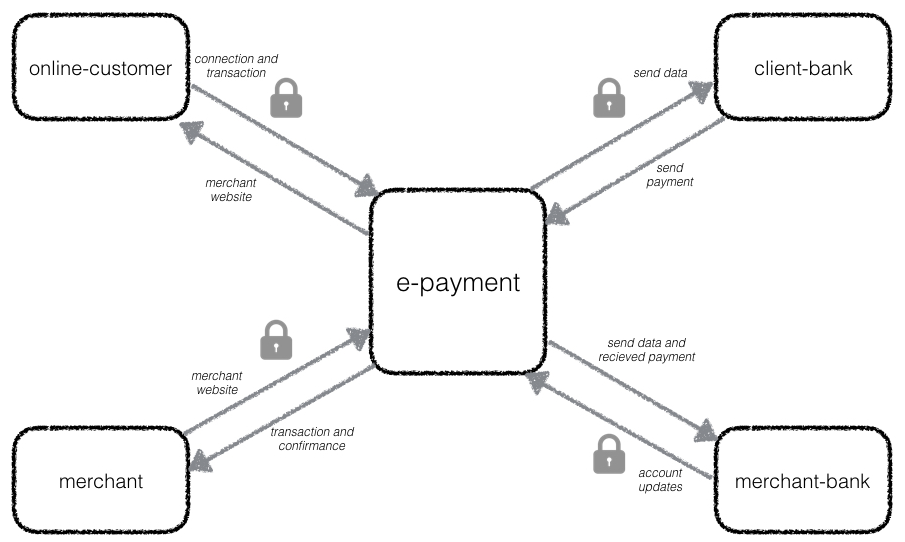
\includegraphics[width=1.0\linewidth]{images/chapter2/payment_model.png}\hfill
\caption[Model of electronic payment gateway]{Model of electronic payment gateway}
\label{fig:model_payment_gateway}
\end{figure}
Where:
\begin{itemize}
\item \emph{online customer}: a customer is an entity who will buy products by
making payments in timely manner;
\item \emph{Merchants}: a merchant is a seller who will receive payments made by customer;
\item \emph{client bank}: client bank holds client’s bank account and validate customer during account registration;
\item \emph{Merchant bank}: merchant bank holds merchant bank account. It is responsible of management, fraud control etc;
\item \emph{payment Gateway}: a payment gateway is connected to all customers, merchants and banks through Internet and responsible for the speed and reliability and security of all transactions that take place.
\end{itemize}
Online Customer will connect to e-payment gateway through Internet. Gateway will connect to the Bank and check whether its bank accounts is enough to buy the required product. Online customer can also visit Merchant’s website through Gateway.
\newline
There are more than 900 payment providers in the world as Briantree, Stripe, Paypal, DataCash, Atos, BPAY, etc. \cite{payment_service_provider}.
\newline
Let's see in the two next sections the first two.